\documentclass[10pt]{article}
\usepackage[polish]{babel}
\usepackage[utf8]{inputenc}
\usepackage[T1]{fontenc}
\usepackage{graphicx}
\usepackage[export]{adjustbox}
\graphicspath{ {./images/} }
\usepackage{amsmath}
\usepackage{amsfonts}
\usepackage{amssymb}
\usepackage[version=4]{mhchem}
\usepackage{stmaryrd}

\title{Zestaw 17 }

\author{}
\date{}


\begin{document}
\maketitle
\begin{center}
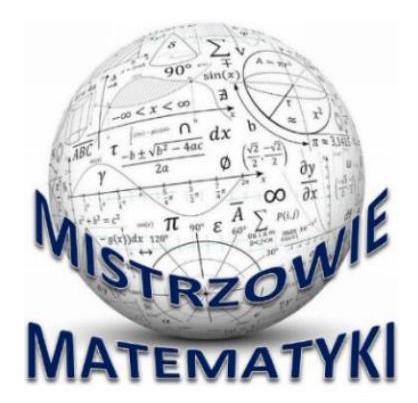
\includegraphics[max width=\textwidth]{2024_11_21_cf2285985aa7c8867f3cg-1}
\end{center}

\begin{enumerate}
  \item Okręgi \(o_{1}\) i \(o_{2}\) przecinają się w punktach \(A\) i \(B\). Prosta \(k\) jest ich wspólną styczną a punkty \(C\) i \(D\) to punkty styczności prostej \(k\) odpowiednio z okręgami \(o_{1}\) i \(o_{2}\). Wykaż, że prosta \(A B\) połowi odcinek \(C D\).
  \item Dwa prostokąty mają jednakowe pola i jednakowe obwody. Wykaż, że mają one również jednakowe przekątne.
  \item Równoległobok \(A B C D\) nie jest prostokątem. Okrąg opisany na trójkącie \(B C D\) przecina przekątną \(A C\) w punkcie \(M \neq C\). Udowodnij, że prosta \(B D\) jest styczna do okręgów opisanych na trójkątach \(A B M\) i \(A D M\).
\end{enumerate}

\end{document}